\documentclass[11pt,a5paper]{article}

\usepackage[T1]{fontenc} % font encoding, lubab õ tähte kasutada
\usepackage[utf8]{inputenc} % oleme siiski 21. sajandis, vajadusel on ka olemas utf8x
\usepackage{lmodern, microtype} % lmodern ja micrtype käivad käsikäes, teeb teksti ilusamaks
\usepackage{enumerate}
\usepackage{caption}
\usepackage[estonian]{babel} % eesti keele poolitamisreeglid jpm
\usepackage[per = fraction, expproduct=cdot, decimalsymbol=comma]{siunitx} % http://www.bakoma-tex.com/doc/latex/siunitx/siunitx.pdf
\usepackage{graphicx} 
\usepackage[european]{circuitikz}
\usepackage{wrapfig}
\usepackage{hyperref}
\usepackage{setspace}
\usepackage{tikz}
\usetikzlibrary{decorations.pathreplacing, positioning}
\usetikzlibrary{arrows,calc,decorations.markings,math,arrows.meta}
\usepackage{siunitx}
\usepackage{epstopdf} %minul on vaja, et .eps pilte saada
%paneme kõik mõõdud paika
\topmargin=-2.5cm \textheight=18cm \textwidth=12.77cm
\oddsidemargin=-1.5cm  \evensidemargin=-1.5cm
\setlength{\parindent}{0pt} \setlength{\parskip}{6pt} \sloppy
\relpenalty=10000 \binoppenalty=10000 % Tekstisisestes valemites reavahetusi ärgu olgu
\pagestyle{empty} % ilma leheküljenumbrita
\newcommand{\numb}[1]{\vspace{5pt}\textbf{\large #1}}
\newcommand{\nimi}[1]{(\textsl{\small #1})}
\newcommand{\punktid}[1]{(\emph{#1~p.})}
\newcommand{\autor}[1]{}
%\newcommand{\autor}[1]{\emph{ Autor: #1}} Temporarily surpressed
\newcounter{ylesanne}
\newcommand{\yl}[1]{\addtocounter{ylesanne}{1}\numb{\theylesanne.} \nimi{#1} \newblock{}}

\begin{document}	
	\begin{center}
		\textbf{\Large Eesti koolinoorte 31. füüsika lahtine võistlus} \par
		\emph{21. november 2020. a. \\Vanema rühma ülesanded (11. - 12. klass)}
	\end{center}
	\resizebox{\textwidth}{!}{%
		\emph{%
			\begin{tabular}{@{}l@{}}
				Lahendamisaeg on 5 tundi. \\
				Iga osavõtja võib lahendada kõiki pakutud ülesandeid. \\
				Arvesse lähevad 6 suurima punktide arvu	saanud lahendust. \\
				Kasutada võib kirjutus- ja joonestusvahendeid ning kalkulaatorit. Muud abivahendid on keelatud.\\
				\textbf{Palun kirjutada iga ülesande lahendus eraldi lehele ning skaneerida eraldi failidesse.}
			\end{tabular}
		}
	}


	\yl{PUDEL}
	Jäigast materjalist pudel (nt klaaspudel) on täidetud osaliselt veega. Rael pani tähele, et väikse pudelikaelaga on pudelist raske kogu vedelikku ära juua. Leidke, mis on maksimaalne vedeliku ruumala, mida on võimalik ära juua ilma pudelisse õhku juurde puhumata. Pudeli ruumala on $V$ ja Rael suudab pudelisse tekitada alarõhu $\Delta P=\num{0.25} p_0$ võrreldes atmosfäärirõhuga, kus $p_0$ on atmosfäärirõhk. Eeldada, et Rael joob vett piisavalt aeglaselt, et pudelis olev õhk on soojuslikus tasakaalus välisõhuga.
	\punktid{6} \autor{Kaarel Kivisalu}
	

	\yl{RUUT FOOKUSES}
	Konstrueerige ruudu $ABCD$ tippude ja külgede kujutised kumerläätses, kui on teada, et
	ruudu keskpunkt $F$ on fookuses ja läätse fookuskaugus on võrdne ruudu
	küljepikkusega ($|AB|=|OF|$, kus $O$ on läätse optiline keskpunkt).
	\punktid{8} \autor{Hannes Kuslap}
	\begin{figure}[h]
		\centering
		\begin{tikzpicture}[scale=0.95]
			\filldraw[black] (-2,0) circle (2pt) node[anchor=south west] {$F$};
			\filldraw[black] (2,0) circle (2pt) node[anchor=south] {$F$};
			\filldraw[black] (0,0) circle (2pt) node[anchor=south west] {$O$};
			\filldraw[black] (-1,1) circle (2pt) node[anchor=south] {$A$};
			\filldraw[black] (-1,-1) circle (2pt) node[anchor=north] {$B$};
			\filldraw[black] (-3,-1) circle (2pt) node[anchor=north] {$C$};
			\filldraw[black] (-3,1) circle (2pt) node[anchor=south] {$D$};
			\draw[gray] [dashed,-] (-4,0) -- (3,0);
			\draw[black, line width=1.5pt] (-1,1) -- (-1,-1);
			\draw[black, line width=1.5pt] (-1,-1) -- (-3,-1);
			\draw[black, line width=1.5pt] (-3,-1) -- (-3,1);
			\draw[black, line width=1.5pt] (-3,1) -- (-1,1);
			\draw[line width=2pt,>=stealth, <->] (0,-2) -- (0,2);
		\end{tikzpicture}
	\end{figure}
	
	
	\vspace{-10pt}
	\begin{wrapfigure}[6]{r}{0.25\linewidth}
		\vspace{-10pt}
		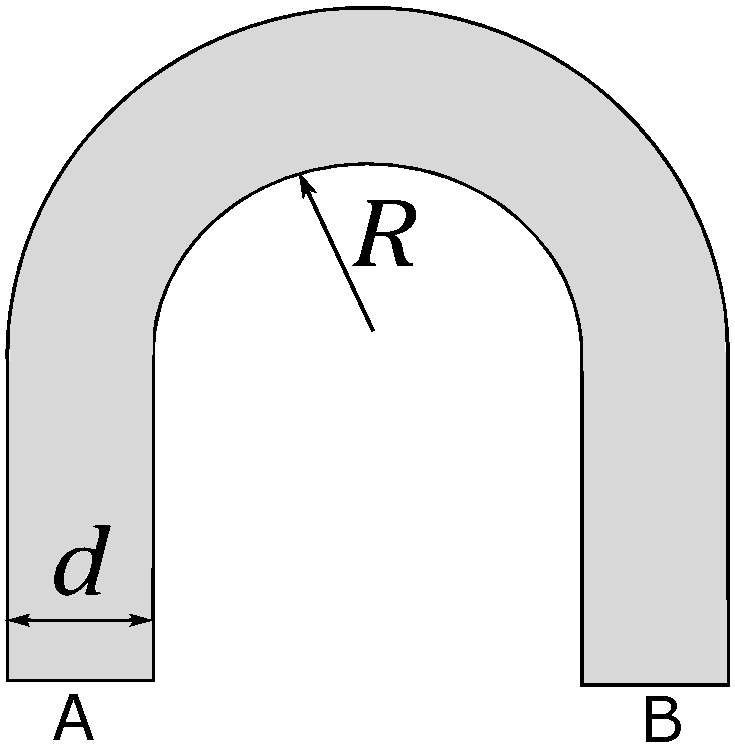
\includegraphics[width=\linewidth]{uklaas_yl.pdf}
	\end{wrapfigure}
	\yl{U-KLAAS} 
	U-kujulise klaastüki (vt joonist) ristlõige on ristkülik. Tahule A langeb selle pinnaga risti paralleelne valgusvihk.  Millist tingimust peaks rahuldama sisemise külje kõverusraadius $R$, et kogu pealelangev valgus väljuks tahust B? Struktuuri laius $d=\SI{3}{\cm}$, klaasi murdumisnäitaja $n=\num{1.5}$ ning tahud A ja B on kaetud peegeldumisvastase kilega.
	\punktid{8} \autor{Hans Daniel Kaimre}
	
	
	\begin{wrapfigure}[12]{r}{0.15\linewidth}
		\vspace{10pt}
		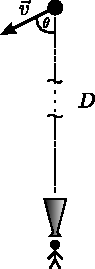
\includegraphics[width=1.1\linewidth]{noova_joon}
	\end{wrapfigure}
	\yl{NOOVA}
	Hobiastronoom Jarl vaatleb teleskoobiga noovaplahvatust ja mõõdab ühe plahvatuse ainejäänuki kiirust. On teada, et ainejäänuki tegelik kiirus on $v$ ja nurk kiirusvektori ja vaatesihi vahel on $\theta$.
	
	Jarl teab varasemate mõõtmiste põhjal, et noova kaugus on $D$, kuid ta ei tea nurka $\theta$. Seetõttu eeldab Jarl, et ainejäänuk liigub vaatesihiga risti ning arvutab kauguse ja jäänuki nurga muutumise abil jäänuki näiva kiiruse $v'$.
	
	Leia Jarli poolt mõõdetav näiv kiirus $v'$, eeldusel et noova on väga kaugel ($vt \ll D$, kus $t$ on vaatluse aeg) ning et kosmoloogiline paisumine on tühine. Valguse kiirus on $c$. Kas on võimalik, et ainejäänuki näiv kiirus $v'$ on mingi $v$ ja $\theta$ väärtuse korral valguse kiirusest suurem, isegi kui $v < c$?
	\punktid{10} \autor{Richard Luhtaru}
	
	
	\yl{SOLENOID JA KONTUUR}
	Pikka solenoidi läbib muutuva tugevusega vool, mille ajaline sõltuvus on näidatud vasakpoolsel joonisel. Solenoidis on $\SI{1}{cm}$ kohta viis keerdu ning solenoidi teljega ristuvas tasandis paikneb parempoolsel joonisel toodud juhtiv kontuur
	eritakistusega $\rho=\SI{1,7e-8}{\Omega.m}$ ja juhtme ristlõikepindalaga $S_0=\SI{2,5}{mm^2}$. Leidke voolutugevuse maksimaalne väärtus kontuuris. Vaakumi magnetiline läbitavus on $\mu_0=\SI{1.26e-6}{H/m}$.
	\punktid{10} \autor{Päivo Simson}
	
	\begin{center}
		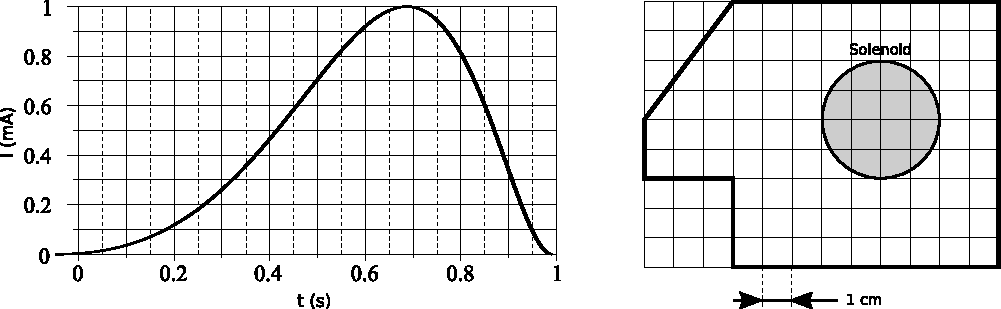
\includegraphics[width=1\linewidth]{induktsioon_joonis.pdf}
	\end{center}


	\newpage
	
	
	\begin{wrapfigure}[8]{r}{0.3\linewidth}
		\vspace{-5pt}
		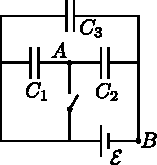
\includegraphics[width=\linewidth]{kondensaator}
	\end{wrapfigure}
	\yl{KONDENSAATORID} Pingeallikas pingega $\mathcal E$ on ühendatud kolme kondensaatoriga mahtuvustega $C_1$, $C_2$ ja $C_3$. Alguses hoitakse lüliti pikalt kinnises olekus. Mitu korda muutub punktide $A$ ja $B$ vaheline pinge peale lüliti avamist ja pika aja möödumist? 
	\punktid{10} \autor{Taavet Kalda}
	
	
	\yl{POOLSILINDER BASSEINIS}\\
	Basseinis laiusega $l$ takistab vedeliku ühelt poolt teisele poole voolamist poolsilinder massiga $m$ ja raadiusega $r$ (ja seega pikkusega $l$), kusjuures telg, piki mida silinder on poolitatud, on vastu basseini põhja. Hõõrdetegur poolisilindri ja basseini põhja vahel on $\mu$, vedeliku tihedus basseinis $\rho$, ja raskuskiirendus on $g$. Basseini üks pool on täidetud veega poolsilindri ülemise ääreni, kõrguseni $r$. Küsimusele vastates eeldage, et hõõrdumine poolsilindri külgmiste poolringide ja seina vahel on tühiselt väike. Mis peaks olema hõõrdeteguri $\mu$ vähim väärtus $\mu_0$, et poolislindri vabastades ei hakkaks see liikuma?
	\punktid{10} \autor{Krister Kasemaa}
	
	
	\yl{TERMOKAAMERA}
	Termokaamera arvutab kehade temperatuure kehadelt saabuva soojuskiirguse intensiivsuse põhjal kasutades koguintensiivsust lainepikkuste vahemikus 7-st kuni 14 mikromeetrini. Antud ülesandes lugegem lihtsustatult, et arvutamiseks kasutatakse koguintensiivsust üle kõigi lainepikkuste (nullist lõpmatuseni). 
	
	Vaskplaadi neeldumistegur on $\varepsilon = \num{0.03}$, st 3\% kogu pealelangevast soojuskiirgusest neeldub ja ülejäänud osa peegeldub. Kui väike vaskplaat asub toas, mis on termodünaamilises tasakaalus (st kõikide kehade temperatuurid on võrdsed toatemperatuuriga $T_0=\SI {20}\celsius$), siis näitab termokaamera õigesti, et vaskplaadi temperatuur on $T_0=\SI {20}\celsius$. Kui aga  vaskplaati kuumutada teatud temperatuurini $T_1$, siis samas toas (endisel temperatuuril) termokaameraga mõõtes saame vaskplaadi temperatuuriks $T_2=\SI {22}\celsius$. Mis on vaskplaadi tegelik temperatuur $T_1$?
	
	\textit{Vihje.} Termodünaamilises tasakaalus oleva keha poolt kiiratav soojuskiirguse koguintensiivsus üle kõigi lainepikkuste on võrdeline neelduvusteguri ja keha absoluutse temperatuuri neljanda astmega (Stefan-Boltzmanni seadus). Absoluutse temperatuuri ja Celsiuse skaala vahe on \SI{273.15}{K}. Termokaamera näit mingi kiirguse korral on võrdne sama palju kiirgava absoluutselt musta keha ($\varepsilon = 1$) temperatuuriga.
	\punktid{12} \autor{Jaan Kalda}

	
	\newpage
	
	\setstretch{0.975}
	
	
	\yl{SUVI}
	Ühel heal päeval kauges tulevikus, kui Maa orbiidi kuju on muutunud, on ta Päikesele
	kõige lähemal suvisel pööripäeval. Sellel suvisel pööripäeval paistab Päike $30\%$
	heledamana kui sama aasta talvisel pööripäeval, s.t. päikesekiirtega risti olevale
	päikesepaneelile langeb $30\%$ võrra suurem kiirgusvõimsus. Mitme päeva võrra erinevad
	selle aasta talve ja suve pikkus ning kumb on pikem? Lugeda, et suvi ja talv algavad
	vastavalt suvisel ja talvisel pööripäeval, s.t. hetkel, mil nurk Maad ja Päikest ühendava
	sirglõigu ning Maa keskpunkti ja põhjapoolust ühendava sirglõigu vahel on vastavalt
	minimaalne või maksimaalne. Suvi ja talv lõpevad hetkel, mil Päikest ja Maad ühendav
	sirge on risti Maa pöörlemisteljega. Eeldada, et aasta jooksul Maa pöörlemistelje suund ei muutu. Maa tiirlemisperiood on $T=\SI{365.26}{päeva}$.
	Atmosfääri efektidega mitte arvestada.\\
	\textit{Vihje.} Kepleri 1. seaduse järgi on planeedi orbiit alati ellips (mida võib käsitleda kui väljavenitatud ringi), kusjuures Päike asub mingis punktis selle pikemal sümmeetriateljel. Kepleri 2. seaduse järgi katab planeeti ja Päikest ühendav sirglõik
	võrdsetes ajavahemikes võrdsed pindalad.
	\punktid{12} \autor{Erik Tamre}
	
	\vspace{-4pt}
	\yl{KOONUS}
	Vabalt painduva venimatu niidi otstes on kuulid massidega $m$ ja $2m$, vt joonist. Kuul massiga $2m$ lebab koonilisel pinnal, mis moodustab horisondiga nurga $\alpha=30^\circ$, raskuskiirendus $g$ on vertikaalselt alla suunatud. Alghetkel on niit pingul ja koonusel lebava kuuli kiirusvektor mooduliga $v_0$ lebab koonuse pinna tasandis moodustades nurga $\beta$ niidiga (st kuuli ja koonuse tippu ühendava sihiga). Teine kuul liigub vertikaalselt niidi pinge ja raskusjõu koosmõjul, algkiirusega $v_0\cos\beta$. Kõiki hõõrdejõude võib ignoreerida.\\
	\osa Kui pika aja pärast  jõuab teine kuul oma teekonna madalaimasse punkti eeldusel, et esimene kuul püsib koonilisel pinnal?\\
	\osa Milline võrratus peab olema rahuldatud, et eelmises punktis tehtud eeldus kehtiks, st et kuulike ei kerkiks kooniliselt pinnalt õhku?
	\punktid{14} \autor{Jaan Kalda}
	
	\begin{center}
		\vspace{-13pt}
		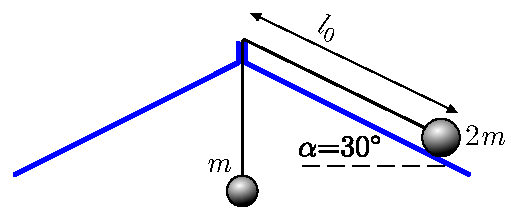
\includegraphics[width=0.55\linewidth]{koonus.pdf}
	\end{center}

\end{document}